\documentclass[12pt, letterpaper]{../assignment}
\usepackage{graphicx}
\usepackage{courier}
\usepackage{minted}
\usepackage{amsmath}
\usepackage{commath}
\usepackage{amssymb}
\usepackage{amsfonts} 
\usepackage{cancel}
\usepackage{enumitem}
\usepackage{array}

\usepackage{tikz}
\usetikzlibrary{shapes,arrows,positioning}

\usemintedstyle{monokai}
\oddsidemargin = 0pt
\exercisesheet{Module 5}{Practice Assignment}
\student{Austin Barrilleaux}
\courselabel{EN 525.609}
\semester{Fall 2023}
\usepackage[backend=bibtex,style=numeric,sorting=none]{biblatex}
\bibliography{reference}
\usepackage{color}
\definecolor{light-gray}{rgb}{0.2,0.2,0.2}
\setminted{bgcolor=light-gray}
\setlength{\parindent}{0pt}

\makeatletter
\patchcmd{\minted@colorbg}{\noindent}{\medskip\noindent}{}{}
\apptocmd{\endminted@colorbg}{\par\medskip}{}{}
\makeatother

\begin{document}
\subsection*{Problem 1}
\subsubsection*{Solve the following practice problems in the 9th edition textbook.\\
\begin{itemize}
    \item Chapter 2:
    \begin{itemize}
        \item 2-33 (a-f)
        \item 2-39 
    \end{itemize}
\end{itemize}}

\subsubsection*{2-33. Without using the Routh-Hurwitz criterion, determine if the following systems are asymp- totically stable. marginally stable, or unstable. In each case, the closed-loop system transfer function is given.}

\subsubsection*{(a) \ \  $ \mathbf{ M(s) = \dfrac{10 (s+2) }{s^3 + 3 s^2 + 5 s}}$}

Using the \texttt{roots()} function MATLAB, we get that the roots are:

$$ \texttt{roots([1,3,4,0])} = \left(\begin{array}{c} 0\\ -1.5000+1.6583{}\mathrm{i}\\ -1.5000-1.6583{}\mathrm{i} \end{array}\right)$$

There is a real pole at $s = 0$.

\begin{answer}
    The system is \textbf{marginally stable}.
\end{answer}

\subsubsection*{(b) \ \  $ \mathbf{ M(s) = \dfrac{(s-1) }{(s+5)(s^2+2)}}$}

Using the \texttt{roots()} function MATLAB, we get that the roots are:

$$ \texttt{roots(conv([1,5],[1,0,2]))} = \left(\begin{array}{c} -5\\ 0.0+1.4142{}\mathrm{i}\\ 0.0-1.4142{}\mathrm{i} \end{array}\right)$$

There are complex conjugate poles on the imaginary axis (real parts of $s$ equal to zero).

\begin{answer}
    The system is \textbf{marginally stable}.
\end{answer}

\subsubsection*{(c) \ \  $ \mathbf{ M(s) = \dfrac{K }{s^3 + 5s + 5}}$}

Using the \texttt{roots()} function MATLAB, we get that the roots are:

$$ \texttt{roots([1,0,5,5])} = \left(\begin{array}{c} 0.4344+2.3593{}\mathrm{i}\\ 0.4344-2.3593{}\mathrm{i}\\ -0.8688 \end{array}\right)$$

There are complex conjugate poles in the right-hand plane (RHP).

\begin{answer}
    The system is \textbf{unstable}.
\end{answer}

\subsubsection*{(d) \ \ $ \mathbf{ M(s) = \dfrac{100(s-1)}{(s+5)(s^2 + 2s + 2)}}$}

Using the \texttt{roots()} function MATLAB, we get that the roots are:

$$ \texttt{roots(conv([1,5],[1,2,2]))} = \left(\begin{array}{c} -5\\ -1+1{}\mathrm{i}\\ -1-1{}\mathrm{i} \end{array}\right)$$

All poles exist in the left-hand plane (LHP).

\begin{answer}
    The system is \textbf{stable}.
\end{answer}

\subsubsection*{(e) \ \ $ \mathbf{ M(s) = \dfrac{100}{s^3 - 2s^2 + 3s + 10}}$}

Using the \texttt{roots()} function MATLAB, we get that the roots are:

$$ \texttt{roots([1,-2,3,10])} = \left(\begin{array}{c} 1.6694+2.1640{}\mathrm{i}\\ 1.6694-2.1640{}\mathrm{i}\\ -1.3387 \end{array}\right)$$

There are complex conjugate poles in the right-hand plane (RHP).

\begin{answer}
    The system is \textbf{unstable}.
\end{answer}


\subsubsection*{(f) \ \ $ \mathbf{ M(s) = \dfrac{10(s + 12.5)}{s^4 + s^3 + 50s^2 + s + 10^6}}$}

Using the \texttt{roots()} function MATLAB, we get that the roots are:

$$ \texttt{roots([1,3,50,1,10\^{}6])} = \left(\begin{array}{c} -22.8487+22.6376{}\mathrm{i}\\ -22.8487-22.6376{}\mathrm{i}\\ 21.3487+22.6023{}\mathrm{i}\\ 21.3487-22.6023{}\mathrm{i} \end{array}\right)$$

There are complex conjugate poles in the right-hand plane (RHP).

\begin{answer}
The system is \textbf{unstable}.
\end{answer}


\subsubsection*{2-39. The loop transfer function of a single-loop feedback control system is given as}

$$ \mathbf{ G(s)H(s) = \frac{K(s+5)}{s (s+2) (1+ T s)} } $$

\subsubsection*{The parameters K and T may be represented in a plane with K as the horizontal axis and T as the vertical axis. Determine the regions in the T-versus-K parameter plane where the closed-loop system is asymptotically stable and where it is unstable. Indicate the boundary on which the system is marginally stable.}

The closed loop transfer function of the above loop transfer function is:

$$ \mathbf{ \frac{G(s)H(s)}{1 + G(s)H(s)} =
\frac{\frac{K(s+5)}{s (s+2) (1+ T s)}}{1+\frac{K(s+5)}{s (s+2) (1+ T s)}} = }
\frac{K(s+5)}{s (s+2) (1+ T s)+ K(s+5)} $$

This makes the characteristic equation:

$$ s (s+2) (1+ T s)+ K(s+5) = 0 $$

Which can be written as:

$$ Ts^3 + (1 + 2T) s^2  + (2 + K)s + 5K  = 0 $$


\begin{center}
    \begin{tabular}{ | m{2em} | m{15em}| m{15em} | } 
      \hline
      $\mathbf{s^3}$ & T & (2 + K) \\ 
      \hline
      $\mathbf{s^2}$ & (1 + 2T) & 5K \\ 
      \hline
      $\mathbf{s^1}$ & $\dfrac{(2 + K)(1 + 2T) -5TK}{(1 + 2T)}$ & 0 \\ 
      \hline
      $\mathbf{s^0}$ & 5K & 0 \\ 
      \hline
    \end{tabular}
\end{center}


The third left-most row is calculated as:

$$ - \frac{\ \left|\begin{array}{cc} T & (2 + K) \\ (1 + 2T) & 5K \end{array}\ \right|}{(1 + 2T)}
 = \dfrac{(2 + K)(1 + 2T) -5TK}{(1 + 2T)}$$

 The fourth left-most row is simply equal to the coefficient of $s^0$.
\\\\
 Given this Routh array, the following must be true so that no signs change occours in the left-most column.

 $$ T > 0 $$

 $$ (T + \frac{1}{2}) > 0 $$

 $$ (2 + K)(1 + 2T) -5TK > 0 $$

 $$ K > 0 $$ 

 Taking $ (2 + K)(1 + 2T) -5TK > 0 $, we can write this as:

 $$ 2 + K + 4T + 2TK -5TK > 0 $$

 Which simplifies to:

 $$ 2 + K + 4T + -3TK > 0 $$

 Solving for K:

 $$ 2 + 4T + K(1-3T) > 0 $$

 $$ 2 + 4T + > K(3T-1) $$

 $$ \frac{(2 + 4T)}{(3T-1)} > K $$

 The condition of stability exists when $ T > 0 $, $ K >0 $ and $ K <\frac{(2 + 4T)}{(3T-1)} $.
 The following figure shows the stability region:

 \begin{figure}[H]
    \centering
    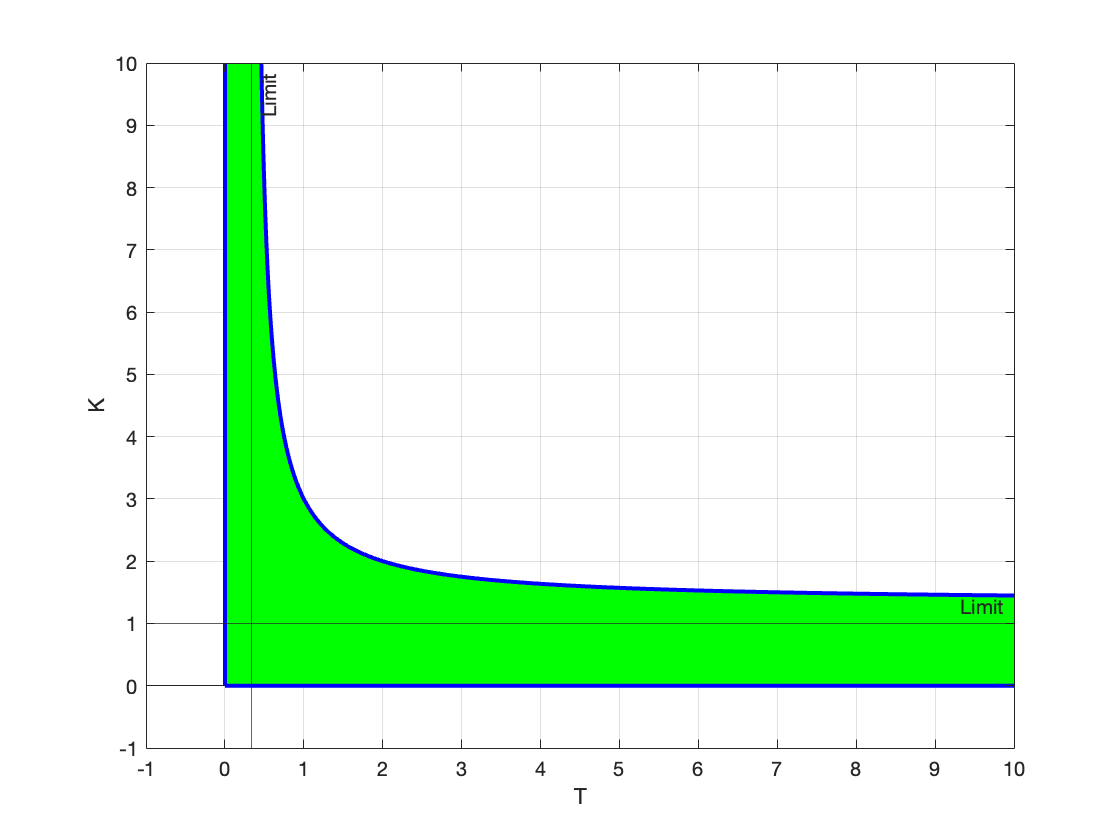
\includegraphics[width=0.7\linewidth]{./figures/stability_region.png}
    \caption{Stability Region}
    \label{fig:stability}
 \end{figure}

 Populating these three boundaries with test values, I can evaluate the roots of the characteristic equation:
\\\\
If I use values of $T =0$ and $K = 1$:
 $$\texttt{roots(subs([T,(1 + 2*T),(2 + K),5*K],[T,K],[0,1]))} =
 \left(\begin{array}{c} -2.5000-2.9580{}\mathrm{i}\\ -2.5000+2.9580{}\mathrm{i} \end{array}\right)$$
\begin{answer}
Indicating that the system is \textbf{stable} along the boundary $T = 0$, since both poles are in the left-hand plane (LHP).
\end{answer}

If I use values of $T =1$ and $K = 0$:
 $$\texttt{roots(subs([T,(1 + 2*T),(2 + K),5*K],[T,K],[1,0]))} =
 \left(\begin{array}{c} -3\\ 0.0-2.2361{}\mathrm{i}\\ 0.0+2.2361{}\mathrm{i} \end{array}\right)$$
\begin{answer}
Indicating that the system is \textbf{marginally stable} along the boundary $K = 0$,
as there are complex conjugate poles with real components equal to zero.
\end{answer}

If we evaluate $ K = \frac{(2 + 4T)}{(3T-1)} $ with the value $T = 2$, we get $K = 2$. Evaluating the characteristic equation with these values:
$$\texttt{roots(subs([T,(1 + 2*T),(2 + K),5*K],[T,K],[2,2]))} =
\left(\begin{array}{c} -2.5000\\ 0.0-1.4142{}\mathrm{i}\\ 0.0+1.4142{}\mathrm{i} \end{array}\right)$$
\begin{answer}
Indicating that the system is \textbf{marginally stable} along the boundary $K = 0$,
as there are complex conjugate poles with real components equal to zero.
\end{answer}

If I use values of $T =0$ and $K = 0$:
 $$\texttt{roots(subs([T,(1 + 2*T),(2 + K),5*K],[T,K],[0,0]))} =
 \left(\begin{array}{c} 0\\ -2 \end{array}\right)$$
\begin{answer}
Indicating that the system is \textbf{marginally stable}at the point $K = 0$ and $T = 0$,
as there is a pole with a value of zero.
\end{answer}



\subsection*{Problem 2}
\subsubsection*{Consider the following transfer function and do the following}
$$ \mathbf{ G(s) = \frac{Y(s)}{R(s)} = \frac{3s+2}{2s^3 + 4s^2 + 5s + 1} } $$
\subsubsection*{(a) Employ the Routh-Hurwitz criterion to determine if this system stable or unstable?}

I wrote the following MATLAB function to solve for a Routh-Array given the coefficients of a characteristic equation:

\color{white}
\hspace*{6em}\inputminted[frame=leftline,fontsize=\footnotesize]{matlab}
{./matlab/routhHurwitz.m}
\color{black}

If I run it using the command \texttt{routhHurwitz([2,4,5,1])}, I get the following result:

\begin{center}
    \begin{tabular}{ | m{2em} | m{15em}| m{15em} | } 
      \hline
      $\mathbf{s^3}$ & 2   & 5 \\ 
      \hline
      $\mathbf{s^2}$ & 4   & 1 \\ 
      \hline
      $\mathbf{s^1}$ & 4.5 & 0 \\ 
      \hline
      $\mathbf{s^0}$ & 1   & 0 \\ 
      \hline
    \end{tabular}
\end{center}

\begin{answer}
Since there are no sign changes in the left-most column, the system is \textbf{stable}.
\end{answer}

If I evaluate the command \texttt{roots([2,4,5,1])} in MATLAB, I get the following:
\\\\
$$ \texttt{roots([2,4,5,1])} = \left(\begin{array}{c} -0.8796+1.1414{}\mathrm{i}\\ -0.8796-1.1414{}\mathrm{i}\\ -0.2408 \end{array}\right)$$

All poles exist in the left-hand plane (LHP).

\begin{answer}
    The system is \textbf{stable}.
\end{answer}

* Note that the function I wrote is not rubust, as if any of the determinants evaluate zero, the resulting table will be incorrect.

\subsubsection*{(b) Define the numerator and denominator in MATLAB, and use the STEP command to plot the system unit step response}

I evaluated the following in MATLAB:

\color{white}
\hspace*{6em}\inputminted[frame=leftline,fontsize=\footnotesize]{matlab}
{./matlab/Problem_2_b.m}
\color{black}

This produced the following plot:

\begin{figure}[H]
    \centering
    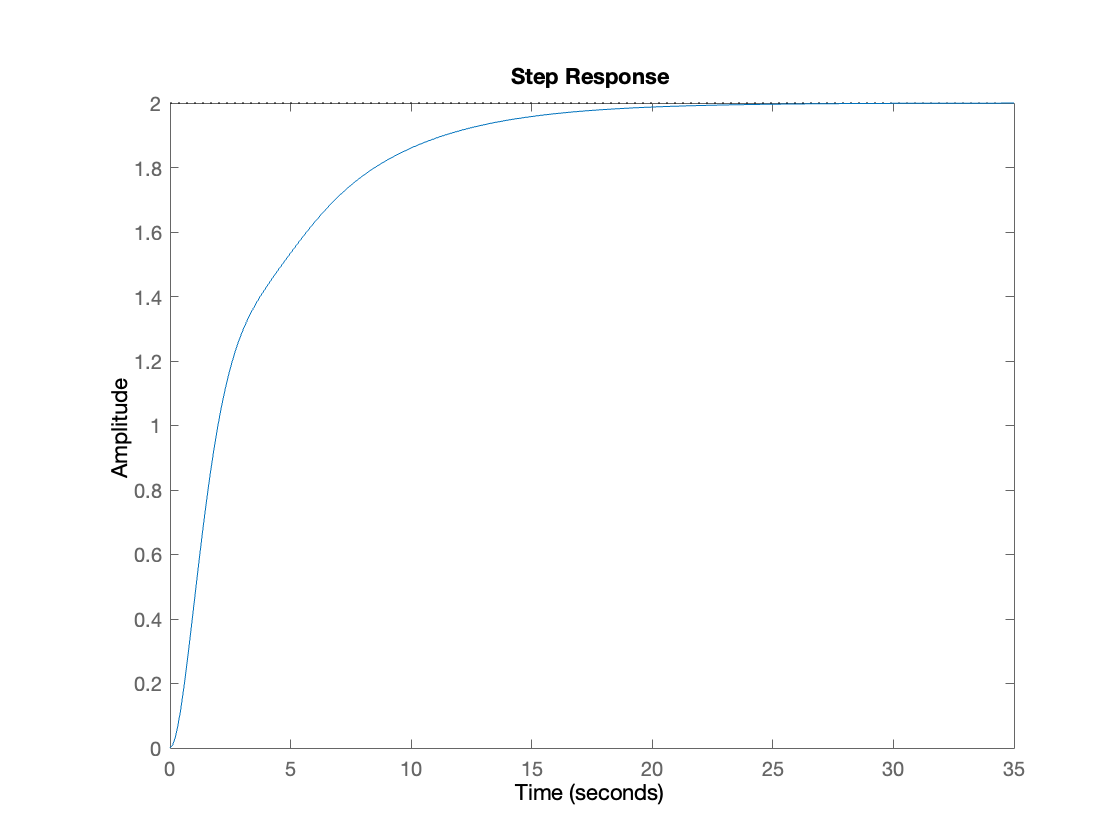
\includegraphics[width=0.7\linewidth]{./figures/step_response.png}
    \caption{Step Response}
    \label{fig:step}
 \end{figure}

\subsubsection*{(c) Use the final value theorem to determine the steady state value of the system - does this agree with the step response?}
    
From the final value theorem we know that:

$$ \lim_{t\to+\infty} f(t) = \lim_{s\to 0} s F(s) $$

Therefore:

$$ \lim_{t\to+\infty} y(t) = \lim_{s\to 0} s Y(s) $$

For the open loop case, given $r(t) = u_s(t) Y$:

$$R(s) = \frac{1}{s}$$

If we substitute this into the closed loop transfer function, we get:

$$ s Y(s) = \frac{3s+2}{2s^3 + 4s^2 + 5s + 1} $$

Therefore:

\begin{answer}
    $$ \lim_{t\to+\infty} y(t) = \lim_{s\to 0} s Y(s) =
        \lim_{s\to 0} \frac{3s+2}{2s^3 + 4s^2 + 5s + 1} = \frac{2}{1} = 2 $$
\end{answer}

\begin{answer}
The steady state value of the system is \textbf{2}, and this \textbf{agrees} with the plot that I produced in part (c).
\end{answer}

\end{document}

